\capitulo{5}{Aspectos relevantes del desarrollo del proyecto}

En este punto de la memoria se van a recoger los aspectos más importantes del desarrollo del proyecto. Se explicarán las decisiones que se tomaron para desarrollar el proyecto de tal forma y los problemas a los que me enfrenté y sus soluciones.

\section{Inicio del proyecto}

Siempre he tenido interés en el deporte, especialmente en el fútbol y me pareció interesante profundizar en como influye la tecnología y la informática en este deporte. \\
El reto de crear una aplicación web dedicada a la consulta de datos y estadísticas de fútbol me atrajo. Sin conocimientos previos en el desarrollo web, me propuse este proyecto como una oportunidad para aprender y desarrollar mis conocimientos de la informática obtenidos en la carrera. A través de este proyecto, he podido explorar y aplicar conceptos de programación, manejo de datos y desarrollo web mientras descubro nuevas cosas sobre el fútbol. Es un trabajo de fin de grado que combina mis gustos personales con mis estudios, permitiéndome crear una herramienta útil y educativa para otras personas aficionadas al deporte. \\
Combinando estas ideas para el trabajo de fin de grado, empecé el desarrollo del mismo. \\
En la figura 5.1 se puede ver el logo de la aplicación web "FutboStats":
\imagen{logo}{Logo de FutboStats}{0.9}

\section{Metodologías}
En el desarrollo del proyecto he utilizado las metodologías ágiles Scrum y Kanban para gestionar y optimizar el flujo de trabajo de manera efectiva.

\subsection{Scrum}
Scrum es un marco de trabajo ágil que se utiliza de forma común en el desarrollo y gestión de proyectos. Esta basado en ciclos de trabajo iterativos e incrementalos llamados \textit{sprints}. Los \textit{sprint} en este proyecto han tenido una duración promedio de dos semanas. Este se consideró el adecuado para poder desarrollar las funcionalidades necesarias de la aplicación. \\
Para llevar a cabo el proceso de Scrum he seguido las siguientes etapas:
\begin{itemize}
    \item \textbf{Planificación del \textit{Sprint}:} al inicio de cada \textit{sprint}, se creaban las nuevas \textit{issues} que se basaban en los objetivos y funcionalidades que se debían completar durante el \textit{sprint}. Cada issue tenía un objetivo claro para garantizar un buen desarrollo. 
    \item \textbf{Ejecución del \textit{Sprint}:} durante el \textit{sprint}, se trabajaban las issues planificadas. La duración de dos semanas me permitían implementar nuevas características a la aplicación y resolver otros problemas que surgían en el proceso.
    \item \textbf{Revisión del \textit{sprint}:} al finalizar el \textit{sprint}, se realizaba una revisión de las issues y de las funcionalidades implementadas. 
    \item \textbf{Planificación del siguiente \textit{Sprint}:} se planificaban las \textit{issues} para el siguiente \textit{sprint}.
\end{itemize}

\subsection{Kanban}
Kanban es una metodología ágil que se centra en la visualización del trabajo y la optimización del flujo de tareas. En el proyecto, se utilizó un tablero Kanban para gestionar y monitorizar las tareas a través de diferentes etapas del proceso de trabajo. \\
En la figura 5.2 se puede ver el tablero Kanban. Este se dividió en varias columnas, cada una representando una etapa del flujo de tabajo:

\imagen{tableroKanban}{Tablero Kanban utilizado en el desarrollo del proyecto.}{1}
\begin{itemize}
    \item \textbf{Por hacer:} esta columna contenía las tareas que aún no se habían iniciado, pero estaban dentro de la planificación del sprint, o para futuros sprints.
    \item \textbf{Listo para hacer:} esta columna contenía las tareas listas para ser comenzadas.
    \item \textbf{En progreso:} las tareas en esta columna se encontraban en desarrollo. 
    \item \textbf{En revisión:} una vez una tarea era completada se movía a esta columna para su posterior revisión. En esta revisión, se comprobaba la calidad del código y la funcionalidad desarrollada. 
    \item \textbf{Hecho:} las tareas que pasaban la revisión se movían finalmente a esta columna, indicando así que estaban completamente terminadas. 
\end{itemize}

El uso combinado de Scrum y Kanban permitió una gestión ágil y eficiente del proyecto, proporcionando un sistema estructurado para la planificación y ejecución de las tareas. Además, este sistema era flexible ante cambios y así permitía optimizar el flujo de trabajo. Con este sistema se aseguró la entrega continua de valor a través de iteraciones incrementales para finalmente llegar al desarrollo completo de la aplicación.

\section{Formación}
Para llevar a cabo este proyecto, se requerían conocimientos técnicos que no disponía al principio. En concreto, se necesitaban ciertos conocimientos avanzados en Angular como la estructurura modularizada, creación de modulos, componentes, servicios, creación de rutas, protección de rutas, conexiones con servicios externos (API-FOOTBALL), conexión con mi API en Flask, como desplegar una aplicación desarrollada en Angular. \\
Para la formación en Angular, se relizó el siguiente curso online:
\begin{itemize}
    \item \textbf{Curso en Udemy:} 'Angular: De cero a experto \cite{udemy:latex}.'
\end{itemize}
Este curso de Udemy ha tenido mucha importancia para llevar a cabo el desarrollo del proyecto, ya que, abarca conocimiento de Angular desde lo más básico de la programación para aprender TypeScript, hasta conceptos avanzados del \textit{framework}. \\
Gracias a este curso intensivo de Angular, he podido aprender a mayor velocidad y aplicar estos conocimientos del curso en la aplicación propuesta.
Los conocimientos que aprendí de Angular en este curso y que aplique en el desarrollo de FutboStats fueron:
\begin{itemize}
    \item Base de TypeScript.
    \item Creación de componentes.
    \item Creación de servicios.
    \item Creación de módulos.
    \item Implementación de Guards.
    \item Implementación de rutas.
    \item Creación y uso de formularios a nivel avanzado.
    \item Estructura modularizada de los proyectos.
    \item Uso de Angular CLI.
    \item Peticiones HTTP.
    \item Utilización de una API externa.
\end{itemize}

Este curso mitiga de gran forma la curva de aprendizaje del \textit{framework}.

\section{Desarrollo de la aplicación}
\subsection{5.4.1 Desarrollo del front-end: Angular}
Una gran parte del proyecto ha sido desarrollar la aplicación web utilizando como \textit{framework} Angular. \\
Antes de iniciar la aplicación, trabaje inicialmente en unos bocetos creados con la aplicación \href{https://www.justinmind.com/?k=just%20in%20mind&a=688685974017&adg=52001997837&cmp=1063145459&match=e&adposition=&utm_medium=cpc&utm_source=google&utm_campaign=1063145459&utm_term=just%20in%20mind_e&gad_source=1&gclid=Cj0KCQjw6auyBhDzARIsALIo6v8LqBRhq_QPIUhxUJt3DHKqPNfvJxZEdrFx4f1jqgqKfJ6g998HKFwaAm_WEALw_wcB}{JustInMind}. Esta aplicación permitía hacer prototipos e incluso simulaciones de los prototipos (ver figura 5.3). De esta forma, asenté las ideas de la aplicación que quería desarrollar. \\
La primera vista que diseñé de la aplicación fue la de pantalla de Inicio, siendo esta la más fácil de todas, ya que no requería conocimientos avanzados. Además, creé la cabecera con el menú de navegación de la aplicación y el pie de la página. Estos primeros pasos me ayudaron a familiarizarme con el \textit{framework}. Cabe destacar, que aunque esta vista fue la primera en diseñarse, ha sido la última en acabarse, ya que se han introducido mejoras para orientar al usuario a como usar la aplicación con pequeños tutoriales introducidos en esta misma vista.
\imagen{prototipo}{Prototipo de la vista de inicio desarrollado en JustInMind}{0.5}

\subsection{5.4.2 Integración de APIs: API-FOOTBALL}
Siguiendo con el desarrollo, me planteé la idea de hacer una vista en la que un usuario pudiera introducir un nombre de una liga y pudiera obtener la clasificación de la misma. Para ello, me puse a investigar sobre APIs externas que pudiera usar y que estuvieran bien documentadas. Finalmente, me decanté por API-FOOTBALL \cite{api:web} debido a las siguientes razones:
\begin{itemize}
    \item \textbf{Amplia cobertura de datos:} proporciona datos detallados y actualizados sobre muchas ligas, competiciones y equipos de fútbol de todo el mundo.
    \item \textbf{Actualizaciones en tiempo real:} ofrece actualizaciones en tiempo real, lo cual es muy importante para aplicaciones que necesitan mostrar información actualizada con frecuencia.
    \item \textbf{Facilidad de integración:} esta diseñada para ser fácil de integrar con distintos tipos de tecnologías de desarrollo web. Angular, proporciona endpoints RESTful que se pueden consumir fácilmente utilizando HTTPClient, lo que facilita la obtención y manipulación en la aplicación. Además, tiene una documentación clara y detallada que ayuda a implementar de forma eficiente las funcionalidades necesarias.
    \item \textbf{Escalabilidad y fiabilidad:} está API está construida para manejar grandes volúmenes de solicitudes, asegurando que la aplicación pueda escalar sin problemas a medida que crece en número de usuarios. La fiabilidad y disponibilidad de la API son esenciales para mantener la integridad de la aplicación y garantizar una experiencia de usuario sin interrupciones.
\end{itemize}
Una vez tenía decidida la API que iba a utilizar y la funcionalidad que quería implementar continué con el desarrollo de la vista llamada 'Competiciones' en la que el usuario podría introducir el nombre de una liga y filtrar por el año para visualizar la clasificación del año que el usuario desease. \\
Como primer problema que tuve que enfrentar fue entender como funcionaban los servicios y las peticiones en Angular utilizando una API externa que requería de una Api-key y de headers como parámetros en la petición http para poder recibir correctamente el JSON que la API me daba como respuesta en función de los parámetros introducidos. \\
Para que el usuario pudiera buscar una clasificación por el nombre de una liga, se creó un servicio con el que a través del nombre de la liga se obtenía el identificador de esa liga. Con ese identificador se llamaría posteriormente al endpoint de clasificaciones para obtener los datos pertenecientes a la clasificación de una liga. Una vez entendí estos conceptos sobre la API y sobre Angular fue sencillo corregirlo y mostrar la información en la web. \\
Una vez estaba implementada la funcionalidad base, trabajé en crear sugerencias interactivas al usuario para que a medida que el usuario introducía el nombre de la liga, aparecieran algunas de las posibles opciones en función de los caracteres introducidos por el usuario (ver figura 5.4). \\
Finalmente, para acabar esta vista implemente mejoras visuales mediante estilos CSS y librerías de Angular tanto en el formulario como en la tabla mostrada. \\
\imagen{sugerencias}{Sugerencias al usuario en la vista 'Competiciones'}{0.4}
Como buenas prácticas de modularización del código, por cada \textit{endpoint} utilizado de la API creé sus interfaces para poder usar el tipado en Angular y un servicio en el cual se hacían las distintas peticiones HTTP para obtener los datos en formato JSON. \\
Fue muy útil utilizar la aplicación Postman para probar las diversas peticiones y entender como funcionaban antes de llevarlas a cabo en Angular. \\

\subsection{5.4.3 Autenticación}
Posteriormente, me pareció interesante implementar un inicio de sesión en la aplicación. En concreto, desarrollé un inicio de sesión con Google utilizando Google Cloud y OAuth2. \\
Para implementar esta parte de la aplicación apliqué los conocimientos del curso de Angular sobre los Guards y las rutas. Los Guards permiten establecer restricciones sobre algunos módulos, como que el usuario no pueda acceder a ellos si no está autenticado en la aplicación. De esta forma los módulos que tuvieran los Guards implementados no se cargarían hasta que el usuario se autenticase en la aplicación. Esto supone una mejora en rendimiento a largo plazo, ya que cuantos menos módulos haya cargados en la aplicación mayor será la escalabilidad del proyecto a largo plazo. Por otro lado, investigué y me leí la documentación de la librería OAuth2 y de Google Cloud para finalizar la implementación del inicio de sesión con Google. Con la librería instalada utilicé sus funciones internas para crear un inicio de sesión y un cierre de sesión. En Google Cloud bastó con crear un nuevo proyecto y especificar la url del proyecto tanto en local como en producción para poder utilizar la funcionalidad en ambas aplicaciones. \\
La figura 5.5 muestra un ejemplo de la configuración de Google Cloud para los dominios en local y producción:
\imagen{googleCloud}{Configuración de rutas en Google Cloud}{0.6}


Por último, plantée una vista que permitiera realizar la búsqueda de partidos a gusto del usuario. Para ello, creé un formulario con los campos nombre de liga, nombre de equipo y fecha. Los únicos parámetros obligatorios para realizar la búsqueda los partidos son el nombre del equipo o el nombre de la liga (uno de ellos o los dos). Si se especifíca uno de ellos, todos los demás son opcionales. Si el usuario realiza mal la búsqueda o introduce una fecha en la que no hay partidos o introduce un nombre de un equipo y liga incompatibles será informado del error, para que pueda corregirlo. \\ 
El calendario que aporta Angular Material viene por defecto en inglés, por lo que utilizando la librería \textit{Moment.js} se realizó el formateado de la fecha a idioma español. Una vez el usuario introduce la fecha, esta debe volver a formatearse a formato inglés para pasarse a la API en la petición, debido a que API-FOOTBALL solo acepta fechas en formato 'MM-DD-YYYY'. \\
Una vez implementada la funcionalidad, el siguiente paso fue mostrar la información de forma ordenada y visual en tarjetas.\\
La figura 5.6 muestra la representación de los partidos buscados por un usuario:
\imagen{partidos}{Ejemplo de búsqueda de partidos del Burgos CF}{1}
Posteriormente, se trabajó en hacer \textit{responsive} todas las pantallas de la aplicación para poder usarla en un dispositivo móvil. Se utilizaron \textit{media-queries} y \textit{flex-layout} para ajustar los componentes de la aplicación. \\
En la figura 5.7 se muestra la vista 'Partidos' adaptada totalmente para dispositivos móviles:

\imagen{responsive}{Adaptación a móvil de FutboStats}{0.3}
 
\subsection{5.4.4 Desarrollo del backend: Flask}
 Otra parte importante del proyecto, fue el desarrollo del back-end con Flask. \\
 Inicialmente, estudié el funcionamiento y la estructura modular de Flask y me creé ficheros de tipo '.ipynb'. En estos ficheros Python desarrollé los modelos de goles esperados (\textit{xG}) y puntos esperados (\textit{xPoints}), así como sus visualizaciones y los distintos gráficos que fui creando con las distintas librerías de Python. Una vez desarrollados, pasaba a implementarlos en la carpeta del proyecto de Flask. \\
 Para desarrollar el modelo de goles esperados (\textit{xG}) creé un '.csv' con los datos de Stastbomb de las 5 grandes ligas europeas (La Liga, Ligue 1, Bundesliga, Premier League, Serie A). \\
 Este '.csv' contenía todos los datos de los eventos de todas las jornadas para todos los equipos. Partiendo de tener los datos en un '.csv' pude desarrollar el modelo de goles esperados. \\
 Debido a que cada vez que se hacía una petición al \textit{back-end} se debía leer un '.csv' de tamaño elevado y ejecutar el modelo, el tiempo de ejecución se elevaba a unos minutos. Para reducir ese tiempo, guardé los resultados finales en un 'JSON'. Este 'JSON' es mandado al \textit{front-end} en Angular para mostrar información del modelo. \\
 Para almacenar las imágenes de gráficos en Flask creé una carpeta llamada 'static'. \\
 Para almacenar los vídeos en Flask creé una carpeta llamada 'uploads'. \\
 El siguiente paso, fue crear las rutas en Flask para poder definir los \textit{endpoints} a los cuáles iba a llamar desde Angular. Aquí, me enfrenté al error 'CORS' (Cross-origin resource sharing), el cual es un error que ocurre cuando se intenta hacer una solicitud http desde una aplicación que se ejecuta en una URL diferente a la del backend. Este problema surge debido a las políticas de seguridad implementadas en los navegadores web para prevenir solicitudes HTTP no autorizadas entre diferentes dominios. \\
 Para su solución en Flask, bastó con instalar la librería '\textit{flaskCors}' de CORS y con ella aplicar una configuración en mi aplicación para permitir solicitudes desde el frontend. \\
 \imagen{cors}{Código empleado para solucionar el problema CORS}{0.5}
 
\subsubsection{Generación de gráficos en Python usando datos de la librería StatsBomb}
Para generar los gráficos en Python utilizando los datos de la librería \textit{StatsBombPy} se han llevado a cabo los siguientes pasos:
\begin{enumerate}
    \item Acceder a los datos de \textit{StatsBombPy} y filtrar dichos datos en función del tipo de gráfico que se quiera crear (datos de jugadores, datos de equipos, datos de una fase eliminatoria). En concreto, se pueden obtener detalles de los partidos de una competición específica como puede ser el mundial de fútbol y filtrar los eventos relacionados con un equipo en particular o una ronda (en la aplicación los gráficos pertenecen a la final del mundial entre Argentina y Francia).
    \item Los datos obtenidos se procesan para extraer la información relevante. Por ejemplo, se filtran los datos para obtener los de un jugador en específico.
    \item Los gráficos han sido creados utilizando la librería \textit{matplotlib}.
\end{enumerate}

Los gráficos creados en el \textit{backend} con Python han sido los siguientes:
\begin{itemize}
    \item \textbf{Mapas de calor:} utilizando los datos de posición de un jugador se muestran las zonas del campo dónde estuvo más activo. Se utiliza la función '\textit{kdeplot}' de \textit{mplsoccer} para crear un gráfico de densidad que resalta las áreas más frecuentadas por el jugador. Con este tipo de gráfico podemos sacar como conclusiones si un jugador tuvo una participación mayormente ofensiva, defensiva o central.

    \imagen{mapaCalorMessi}{Ejemplo de mapa de calor generado en Python.}{0.8}

    \item \textbf{Mapas de posiciones:} utilizando los datos de las coordenadas en las que un jugador estuvo en el campo se puede crear un gráfico que refleja todas las coordenadas mostrando si un jugador fue más ofensivo o defensivo. Con este tipo de gráfico podemos comprobar si un jugador estuvo presente en muchas zonas del campo, es decir, estuvo presente en recuperaciones de balón, atacando, defendiendo.

    \imagen{mapaPosiciones}{Ejemplo de mapa de posiciones de un jugador generado en Python.}{0.8}

    \item \textbf{Mapas de pases:} utilizando los datos de los pases de un jugador se pueden crear gráficos que muestren las trayectorias de los pases. Los pases en verde reflejan pases que tuvieron éxito en la entrega a otro jugador. En cambio, los pases en rojo son aquellos que no se entregaron correctamente. Este gráfico nos presenta una posible tendencia del jugador en el momento de hacer los pases y en que zonas suele acertar o fallar los pases.

    \imagen{mapaPases}{Ejemplo de mapa de pases de un jugador generado en Python.}{0.8}

    \item \textbf{\textit{Match momentum}}: este gráfico utiliza los datos de los eventos de un partido como pases, conducciones de balón, disparos, goles. Se genera un gráfico que muestra de forma gráfica que equipo dominó en cada momento del partidos, observando si los goles llegaron en un momento bueno o malo del equipo.

    \imagen{matchMomentum}{Ejemplo de gráfico \textit{match momentum} generado en Python.}{0.8}

    \item \textbf{Portería:} con los datos de los disparos (acabaran en gol o no) de un partido se puede crear un gráfico que representa una portería dividida en secciones y muestra los lugares en los que un equipo disparó más o tuvo mayor probabilidad de gol.

    \imagen{graficoPorteria}{Ejemplo de gráfico de una portería que representa los disparos que tuvo Argentina en el mundial 2022.}{0.8}
\end{itemize}

 \subsubsection{Integración de ImageAI}
 Siguiendo con el desarrollo del \textit{back-end}, cabe destacar la implementación de imageAI, la cual no fue complicada gracias a la documentación de la librería. Una vez conseguí el vídeo procesado por el algoritmo, surgió el problema al intentar enviarlo al front-end. \\
 Este error consistía en que el vídeo perdía las propiedades de su codec al ser procesado por el algoritmo. Para solucionar este error, utilicé la herramienta \textit{Ffmpeg}, la cual se puede instalar en cualquier sistema operativo y se puede configurar en las variables de entorno del sistema para que pueda ser accesible a través de cualquier script en Python. Con esta herramienta, seguí el siguiente proceso para obtener el vídeo final:
 
\begin{itemize}
    \item Procesar vídeo elegido
    \item Guardar resultado del procesamiento con imageAI en un fichero temporal en la carpeta 'uploads'.
    \item Utilizar \textit{Ffmpeg} con el fichero temporal para generar el fichero de vídeo final.
    \item Obtener el fichero de vídeo final con el codec correcto y guardarlo en la carpeta uploads.
\end{itemize}
Posteriormente, realicé la conexión de Angular con Flask de esta funcionalidad. Desde Angular, un usuario hace un POST de un fichero '.mp4' a Flask. Este fichero es procesado en el back y devuelto al front para su visualización posterior. El usuario puede a través del reproductor utilizado descargar el vídeo.

\subsection{Arquitectura en local}
La figura 5.9 muestra un esquema de la arquitectura de la aplicación a nivel local:
\imagen{esquemaLocal}{Arquitectura de la aplicación en local}{0.9}
En el esquema podemos ver como la aplicación en local se compone de Angular y Flask, los cuáles se pasan datos a través de peticiones GET y POST. Desde Angular se hacen peticiones GET a API-FOOTBALL que nos devuelve en ela respuesta un JSON. Finalmente, he representado las carpetas uploads y static que utilizo en el back para guardar los ficheros que se muestran en front-end.

\section{Despliegue de la aplicación}
Una vez la aplicación desarrolló completamente las funcionalidades pasó a desplegarse a producción para su uso. El \textit{front-end} en Angular se desplegó en \href{https://www.netlify.com/}{Netlify}, mientras que el \textit{back-end} en Flask se desplegó en \href{https://render.com//}{Render}.
El despligue en Netlify no supuso mayores problemas que seguir los pasos indicados. En cambio, el despligue en Render tuvo algunos problemas debido a conflictos de dependencias en el fichero 'requirements.txt' que Render utilizaba para configurar el proyecto. Este error fue solucionado actualizando las dependencias que daban errores. Cabe destacar que la funcionalidad de los vídeos que consiste en que un usuario haga un POST al \textit{back-end} de un vídeo para obtener de vuelta el mismo procesado por el algoritmo de imageAI no funciona debido a que los recursos que proporciona la versión gratuita de Render son escasos y no soporta la transferencia de archivos de gran volumen, además de permitir bajos recursos en uso de CPU y memoria RAM. Por ello, se aportará junto con el proyecto una máquina virtual con instrucciones para poder utilizar esta funcionalidad y toda la aplicación en local. 

\imagen{despliegue}{FutboStats desplegada en Netlify y Render}{0.9}

A continuación, muestro un esquema de la arquitectua de la aplicación a nivel de producción:

\imagen{arquitecturaDespliegue}{Arquitectura de la aplicación en producción.}{1}
\section{Testing}
Las pruebas que realicé en mi aplicación fueron utilizando la herramienta Postman. \\
He utilizado esta herramienta para probar los endpoints de las APIs utilizadas en el proyecto (API-FOOTBALL y API en Flask) antes de implementar los servicios que contendrían estas llamadas en Angular. \\
Utilicé Postman por las siguientes razones:
\begin{enumerate}
    \item Postman ofrece una interfaz de usuario amigable que facilita la creación, configuración y prueba de solicitudes HTTP sin necesidad de escribir código adicional. Esto permite a los desarrolladores centrarse en la lógica de la API.
    \item Es sencillo configurar todos los aspectos de una solicitud HTTP, como el método (GET, POST, PUT, DELETE), los headers (\textit{api-key}, \textit{api-host}), parámetros de consulta, el cuerpo de la solicitud, autenticación. Esto permite replicar exactamente las condiciones que la API esperaría en producción.
    \item Postman permite probar rápidamente diferentes endpoints de una API y validar las respuestas. Se pueden ver las respuestas de la API en formato JSON, XML o texto plano, lo que facilita la comprobación de que los datos devueltos son correctos y están en el formato esperado.
    \item Soporta la creación de entornos (desarrollo, prueba, producción), cada uno con sus propias variables de entorno como URL base, claves API.
\end{enumerate}

\subsection{Ejemplo de uso de Postman: API-FOOTBALL}
Las solicitudes a la API-FOOTBALL se estructuran en formato JSON y contienen parámetros como el nombre del equipo, nombre de la liga o fecha del partido. Estas solicitudes requieren incluir una clave de API llamada (\textit{API key}) y un host de API llamado (\textit{API host}) en los encabezados para autenticación. Cada \textit{endpoint} de la API tiene parámetros establecidos, algunos de los cuales son opcionales.
Para acceder a API-FOOTBALL, es necesario incluir en cada solicitud los siguientes encabezados:
\begin{itemize}
    \item \textbf{API key:} Clave única proporcionada al registrarse en API-FOOTBALL, utilizada para autenticar las solicitudes.
    \item \textbf{API host:} Identificador del host de la API, que especifica el servidor al cual se envían las solicitudes.
\end{itemize}
Cada \textit{endpoint} de la API-FOOTBALL acepta diferentes parámetros, que pueden ser obligatorios u opcionales. Algunos de los parámetros comunes incluyen:
\begin{itemize}
    \item \textbf{Identificador del equipo:} identificador del equipo para el cual se desean obtener datos.
    \item \textbf{Identificador de la liga:} identificador de la liga para la cual se quieren obtener estadísticas o clasificaciones.
    \item \textbf{Fecha:} fecha del partido para el cual se desean obtener los resultados o detalles.
    \item \textbf{Season:} año de la temporada por la que se desea filtrar la información.
\end{itemize}

\begin{figure}[H]
    \centering
    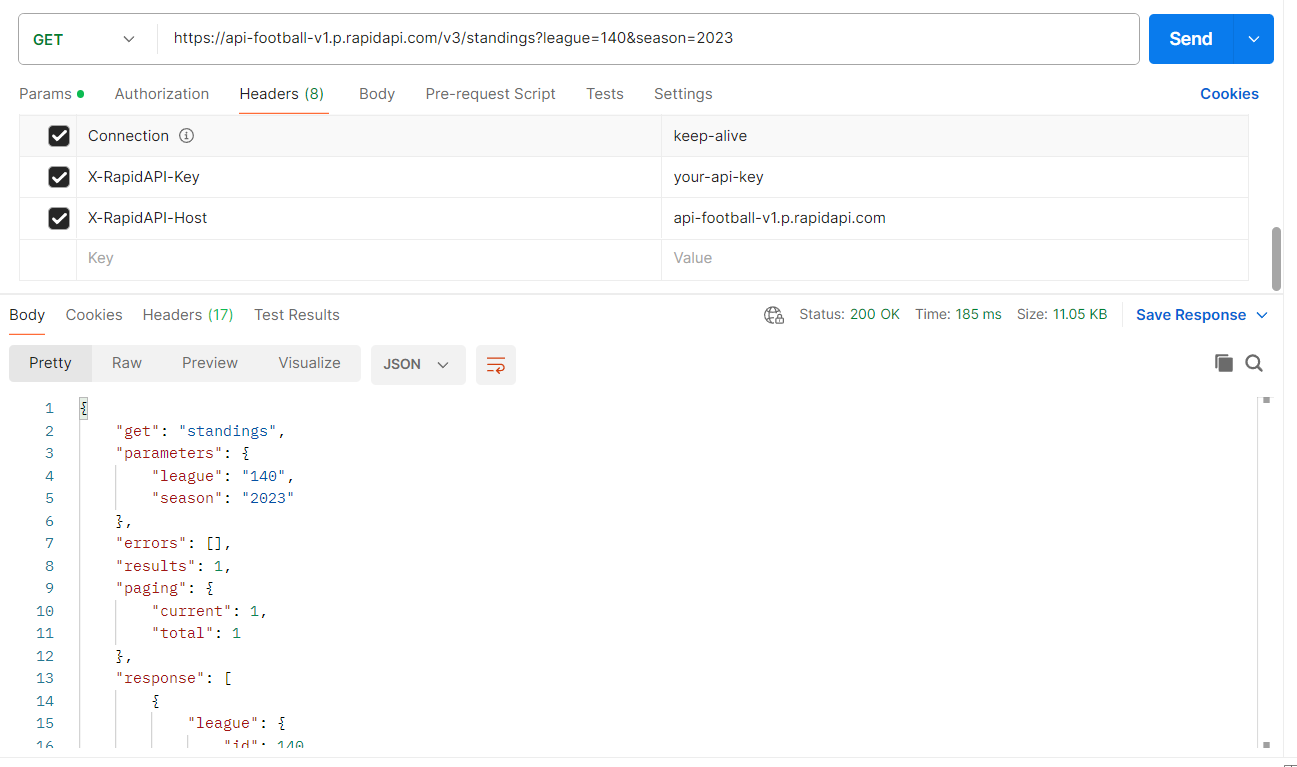
\includegraphics[width=1\linewidth]{img/ejemploPostman.png}
    \caption{Ejemplo de petición a API-FOOTBALL}
    \label{fig:enter-label}
\end{figure}

Como podemos ver en la figura 5.17 se realiza una petición GET al endpoint '/standings' para obtener una clasificación en concreto. Le pasamos como parámetros el identificador de liga 140 (es el identificador de La Liga española) y la season 2023 (año de la clasificación). Para que la petición tenga éxito tenemos que establecer en los headers el campo 'X-RapidAPI-Key' con la Api-key que da API-FOOTBALL al registrarse y el campo 'X-RapidAPI-Host' con el host correspondiente que en mi caso es 'api-football-v1.p.rapidapi.com'. Como podemos observar en el \textit{body} tenemos el resultado en JSON de la petición GET y el status de la petición (200 OK).

\subsection{Estructura de solicitudes y respuestas de la API en Flask}
La API diseñada en Flask contiene varios endpoints. Algunos devuelven un JSON con la información del modelo de goles esperados, información de la tablas de los puntos esperados. En cambio, otros devuelven gráficos generados en Python utilizando los datos de \textit{StatsbombPy}.\\

\begin{figure}[H]
    \centering
    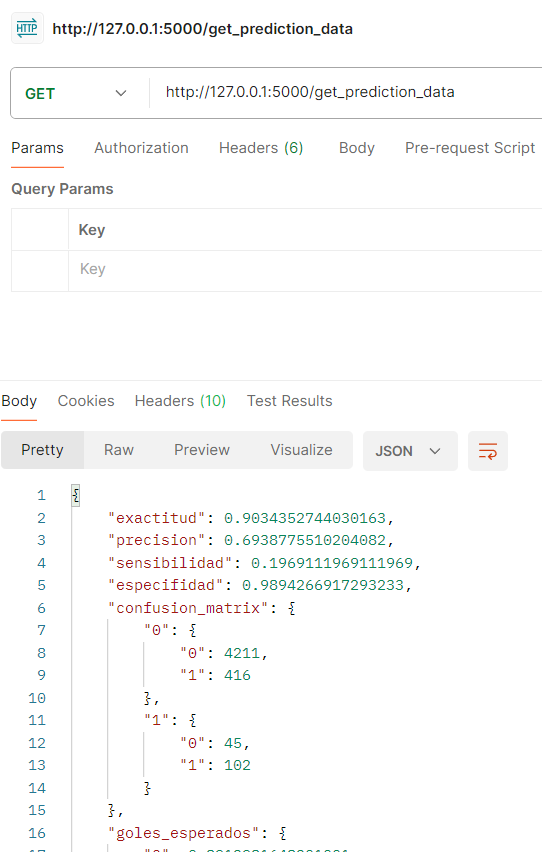
\includegraphics[width=0.5\linewidth]{img/ejemploPostmanAPIFlask.png}
    \caption{Ejemplo de petición a la API de Flask}
    \label{fig:enter-label}
\end{figure}

Como podemos ver en la figura 5.18, se realiza una petición a un \textit{endpoint} que devuelve un JSON con la información del modelo de goles esperados que se mostrará en el \textit{front-end} en forma de tarjetas.
